% \input{\pSections "sec-results"}

\section{Results in 2D}
%     %     %     %     %     %     %     %     %
\subsection{Scanning an Object}
\begin{frame}{Mercury MoM Sweeps Frequencies and Orientation}
    \centering
    \begin{overpic}[width=\textwidth]{\pLocalGraphics/fiducial-ptw-rcs.pdf}
        % Add annotations with \put(x,y){content}
        %\put(20,85){\color{red}\textbf{Important Feature}}
        %\put(50,50){\includegraphics[width=2cm]{\pLocalGraphics/arrow.pdf}}
        %\put(10,10){\color{blue}\textit{Additional Note Here}}
    \end{overpic}
    \vspace{0.5cm}
    %\textit{Figure: Annotated visualization of the fiducial PTW RCS data.}
\end{frame}

\begin{frame}{Follow-on Notes: Mercury MoM Sweeps}
    \begin{itemize}
        \item \textbf{Sweep Overview:}
        \begin{itemize}
            \item OTHR Frequency range: $[3, 30]$ MHz.
            \item Wavelength: $[100, 10]$ m.
           %\item Orientation varies: X-axis represents azimuth.
            \item Color represents \textbf{return energy levels}
        \end{itemize}
        \item \textbf{Azimuth Details:}
        \begin{itemize}
            \item Azimuth range: $[0^\circ, 360^\circ]$.
            \begin{itemize}
                \item $0^\circ$: Nose on.
                \item $-90^\circ$: Copilot side.
                \item $90^\circ$: Pilot side.
                \item $180^\circ$: Tail on.
            \end{itemize}
        \end{itemize}
    \end{itemize}
\end{frame}

\begin{frame}{Frequency Notes and Plot Interpretation}
    \begin{itemize}
        \item \textbf{Frequency Notes:}
        \begin{itemize}
            \item Resonance peaks identified at key frequencies in red.
            \item Highlighted transitions between modes for particular azimuths.
        \end{itemize}
        \item \textbf{Plot Interpretation:}
        \begin{itemize}
            \item MoM will sweep frequencies.
            \item MoM will sweep orientation.
            \item MoM is ready for 3D.
        \end{itemize}
        \item \textbf{Resolution}
        \begin{itemize}
            \item At 3 Mhz (100 m) target is fuzzy.
            \item At 30 Mhz (10 m) features appear.
        \end{itemize}
    \end{itemize}
\end{frame}


%     %     %     %     %     %     %     %     %
\subsection{Fidelity of Approximation}
\begin{frame}{Fourier Transform Visualizations at 16 MHz}
    \centering
    \begin{tabular}{ccc}
        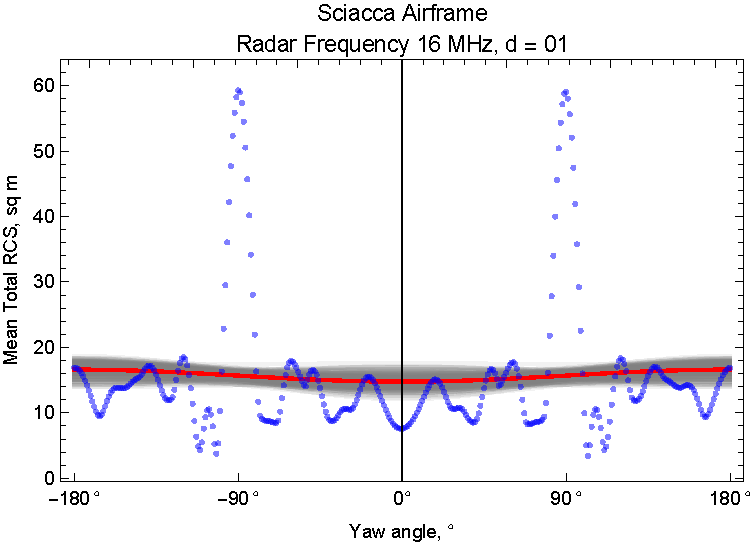
\includegraphics[ width = 0.3\textwidth ]{ \pLocalGraphics/wh-fourier-16Mhz-d01.pdf } & 
        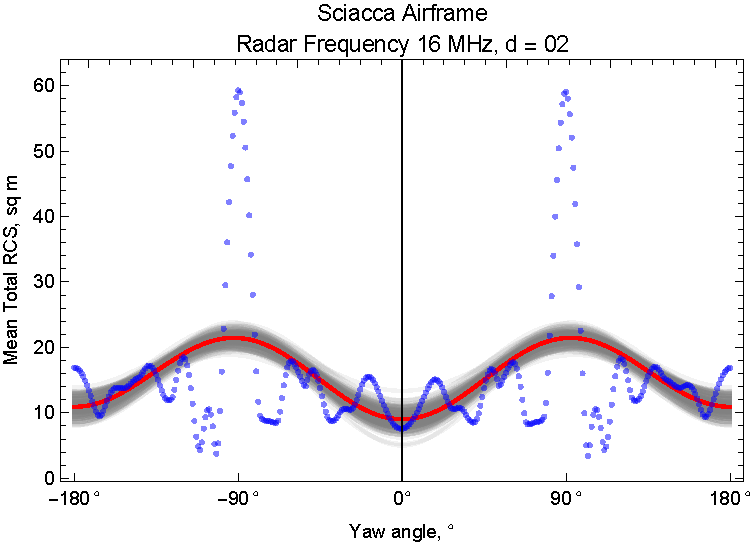
\includegraphics[ width = 0.3\textwidth ]{ \pLocalGraphics/wh-fourier-16Mhz-d02.pdf } & 
        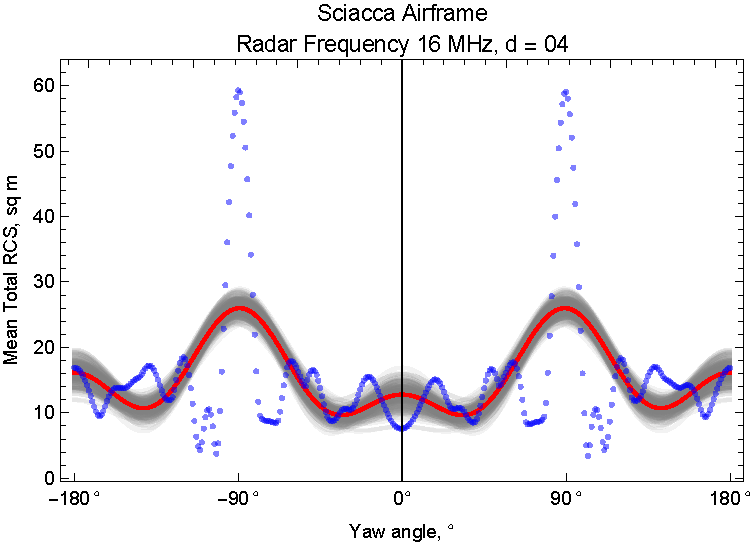
\includegraphics[ width = 0.3\textwidth ]{ \pLocalGraphics/wh-fourier-16Mhz-d04.pdf } \\
        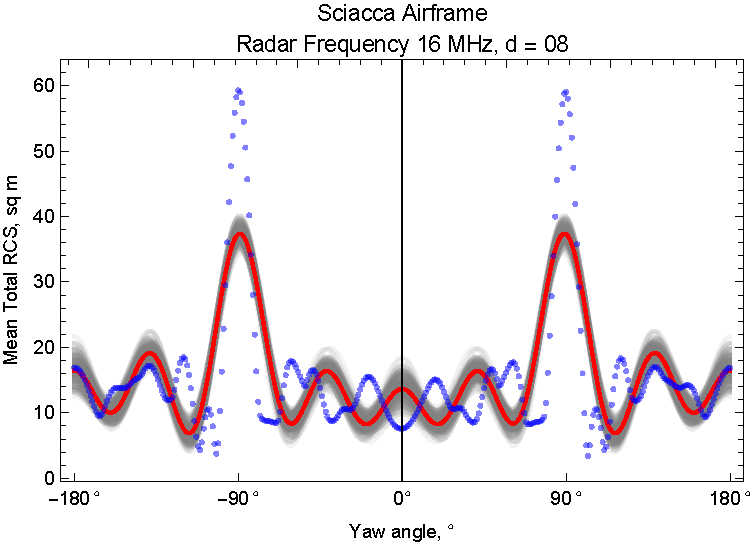
\includegraphics[ width = 0.3\textwidth ]{ \pLocalGraphics/wh-fourier-16Mhz-d08.pdf } & 
        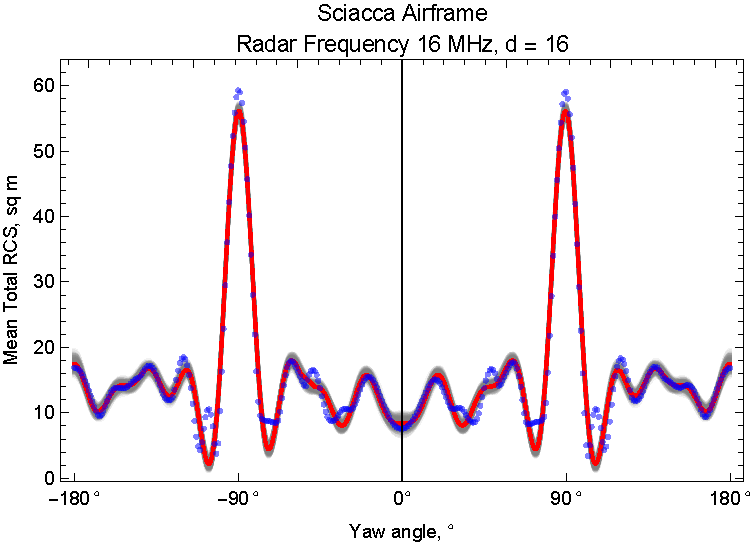
\includegraphics[ width = 0.3\textwidth ]{ \pLocalGraphics/wh-fourier-16Mhz-d16.pdf } & 
        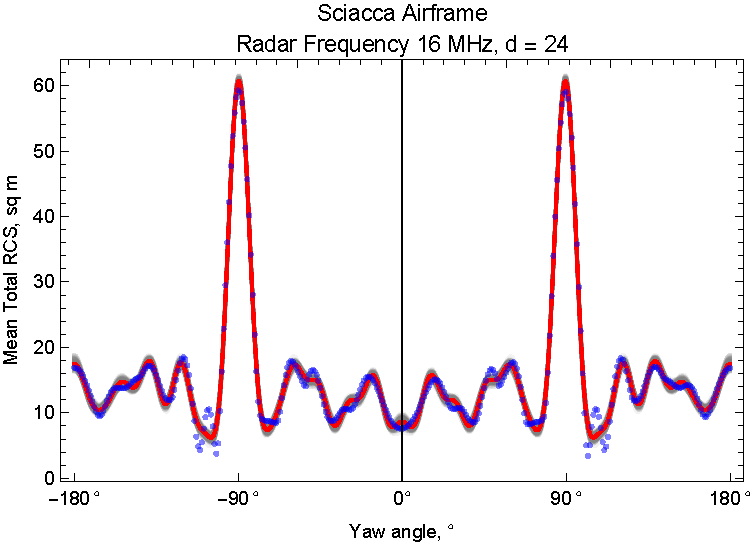
\includegraphics[ width = 0.3\textwidth ]{ \pLocalGraphics/wh-fourier-16Mhz-d24.pdf } \\
    \end{tabular}
    \vspace{0.0em}
    %\caption{Visualizations of the Fourier Transform at 16 MHz for Different Parameters.}
    \begin{block}{\centering \footnotesize Note}
         \footnotesize {\textcolor{blue}{Blue:} Data \hspace{1em} \textcolor{red}{Red:} Approximation \hspace{1em} \textcolor{gray}{Gray:} Error}
    \end{block}
    \label{tab:fidelity}
\end{frame}

\begin{frame}{A Closer Look A Fits and Errors 1/3}
    \centering
\begin{table}[htp]
%\caption{default}
\begin{center}
\begin{tabular}{cccc}
			%
	$d$ & Data Fit & Residual Error & Total Error \\\hline
			%
        \raisebox{1cm}{$0$} &
        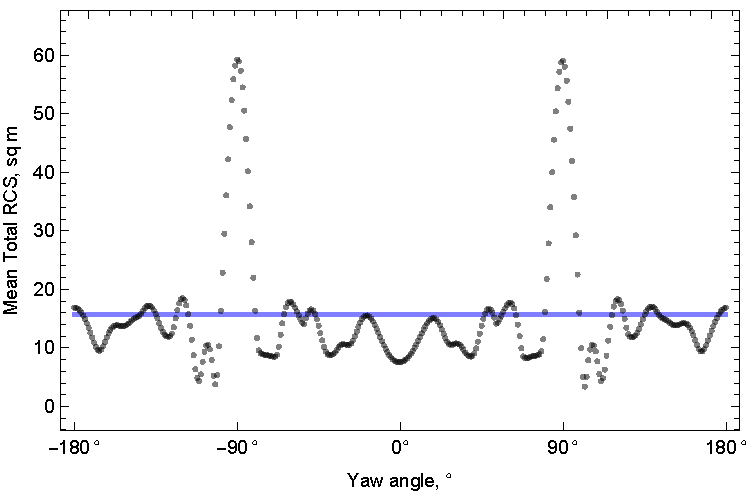
\includegraphics[width=3.1cm]{\pLocalGraphics/nu/nu=16-d=00-A} &
        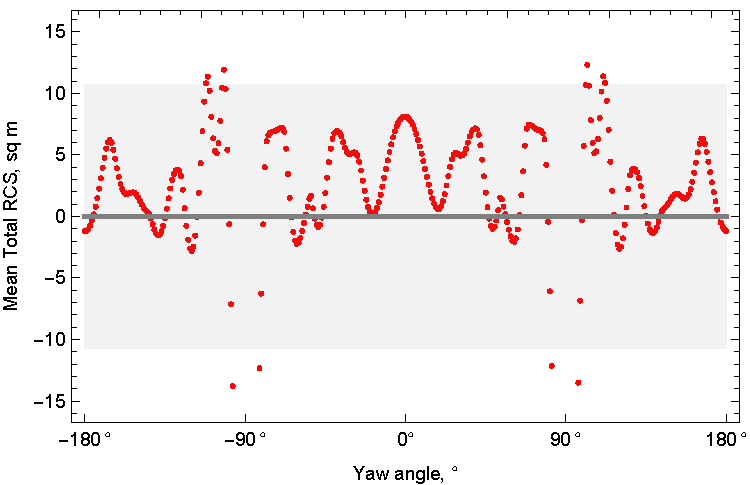
\includegraphics[width=3.1cm]{\pLocalGraphics/nu/nu=16-d=00-B} &
        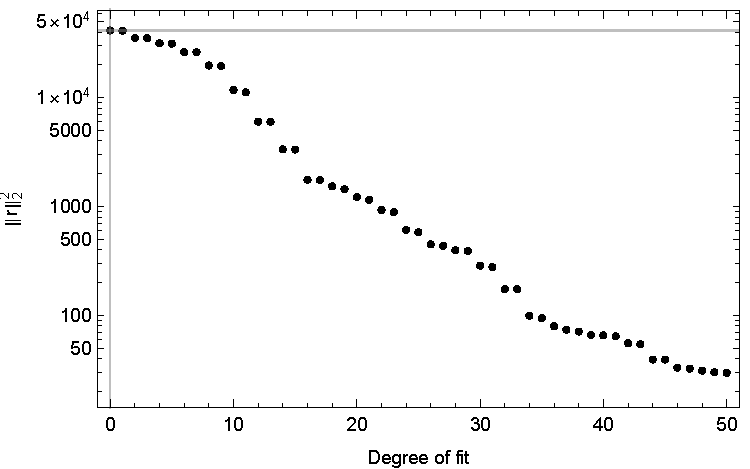
\includegraphics[width=3.2cm]{\pLocalGraphics/nu/nu=16-d=00-C} \\
			%
        \raisebox{1cm}{$2$} &
        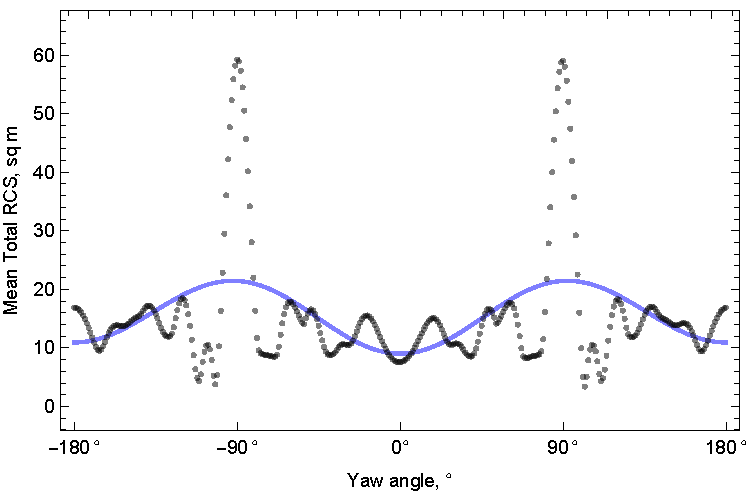
\includegraphics[width=3.1cm]{\pLocalGraphics/nu/nu=16-d=02-A} &
        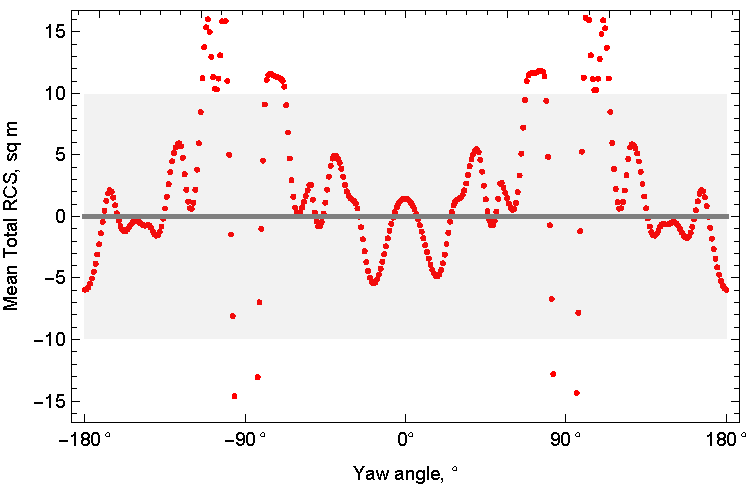
\includegraphics[width=3.1cm]{\pLocalGraphics/nu/nu=16-d=02-B} &
        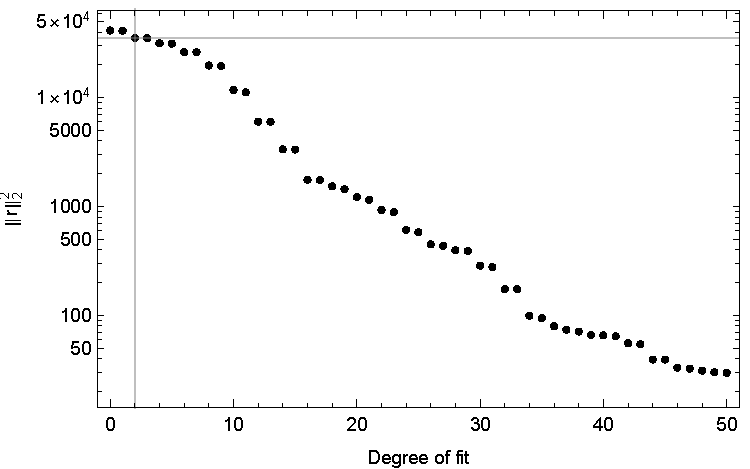
\includegraphics[width=3.2cm]{\pLocalGraphics/nu/nu=16-d=02-C} \\
			%
\end{tabular}
\end{center}
\label{tab:a}
\end{table}%
\end{frame}

\begin{frame}{A Closer Look A Fits and Errors 2/3}
    \centering
\begin{table}[htp]
%\caption{default}
\begin{center}
\begin{tabular}{cccc}
			%
	$d$ & Data Fit & Residual Error & Total Error \\\hline
			%
        \raisebox{1cm}{$4$} &
        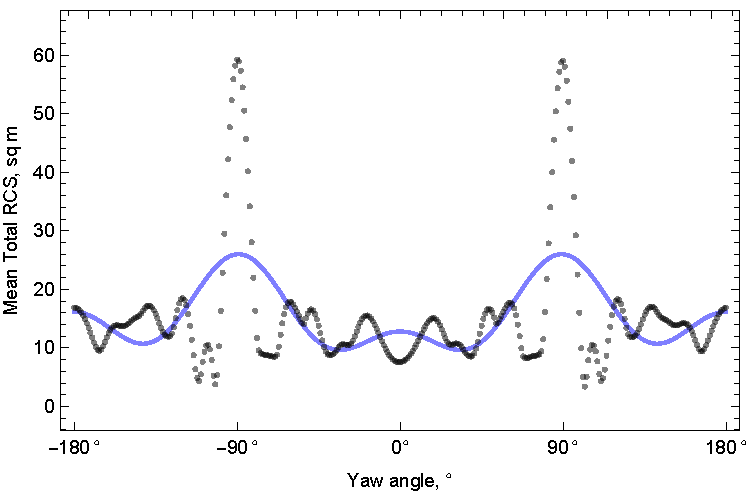
\includegraphics[width=3.1cm]{\pLocalGraphics/nu/nu=16-d=04-A} &
        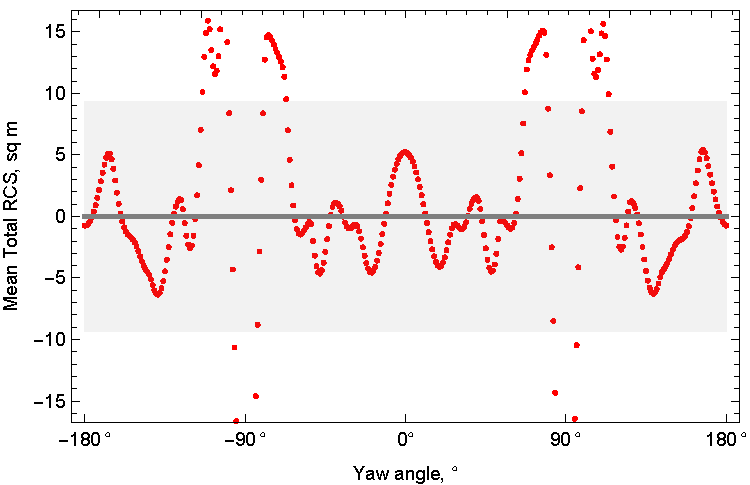
\includegraphics[width=3.1cm]{\pLocalGraphics/nu/nu=16-d=04-B} &
        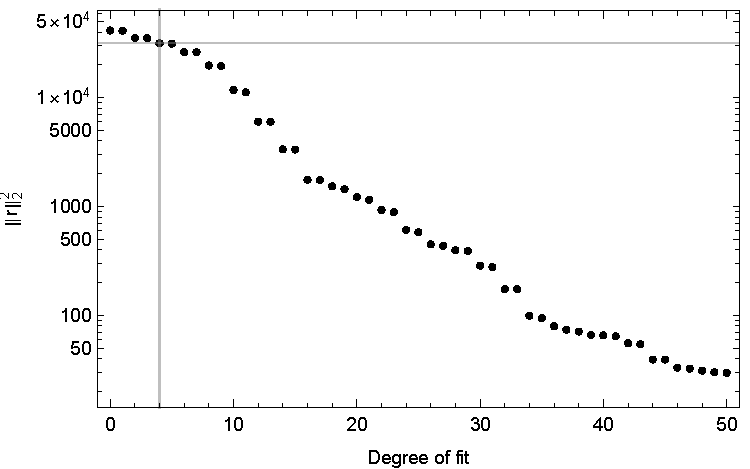
\includegraphics[width=3.2cm]{\pLocalGraphics/nu/nu=16-d=04-C} \\
			%
        \raisebox{1cm}{$8$} &
        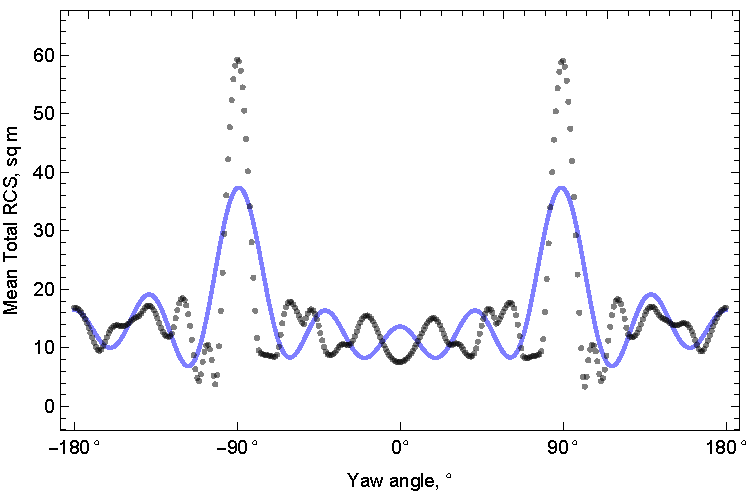
\includegraphics[width=3.1cm]{\pLocalGraphics/nu/nu=16-d=08-A} &
        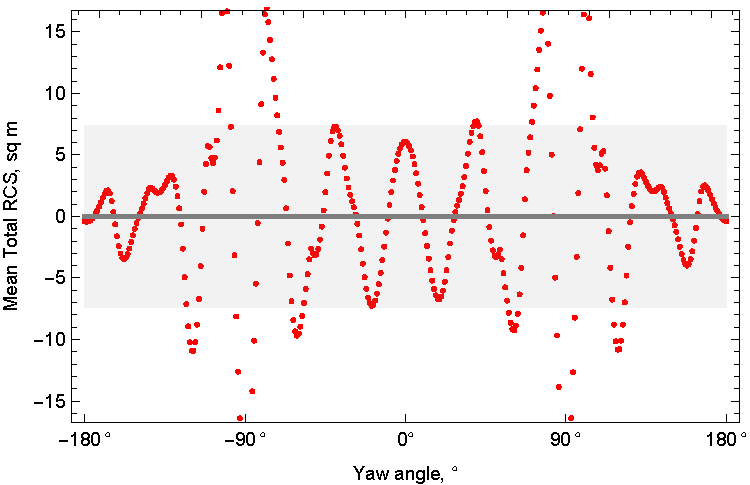
\includegraphics[width=3.1cm]{\pLocalGraphics/nu/nu=16-d=08-B} &
        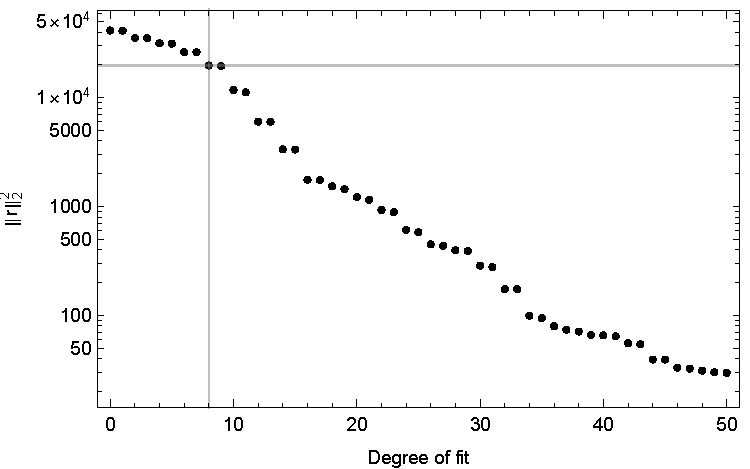
\includegraphics[width=3.2cm]{\pLocalGraphics/nu/nu=16-d=08-C} \\
			%
\end{tabular}
\end{center}
\label{tab:b}
\end{table}%
\end{frame}


\begin{frame}{A Closer Look A Fits and Errors 3/3}
    \centering
\begin{table}[htp]
%\caption{default}
\begin{center}
\begin{tabular}{cccc}
			%
	$d$ & Data Fit & Residual Error & Total Error \\\hline
			%
        \raisebox{1cm}{$16$} &
        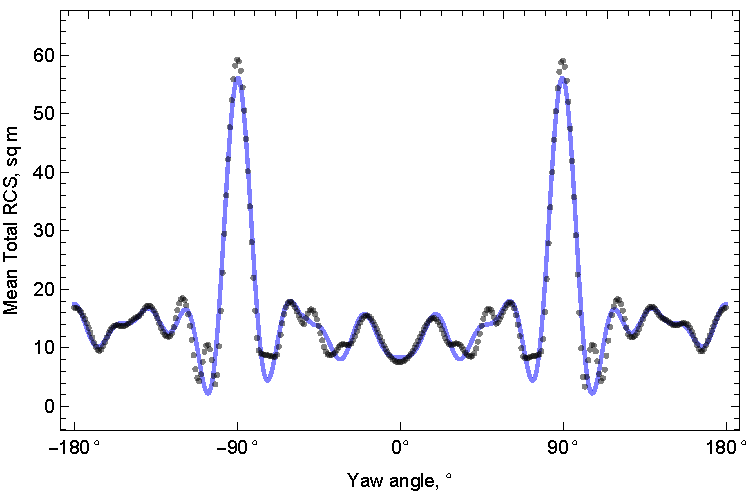
\includegraphics[width=3.1cm]{\pLocalGraphics/nu/nu=16-d=16-A} &
        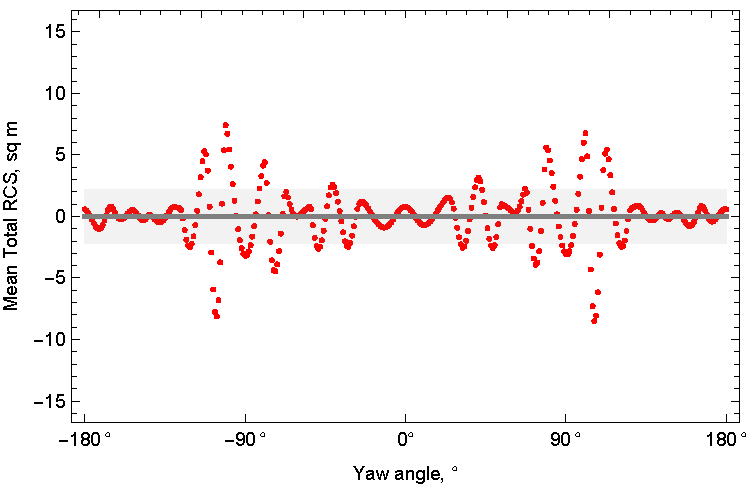
\includegraphics[width=3.1cm]{\pLocalGraphics/nu/nu=16-d=16-B} &
        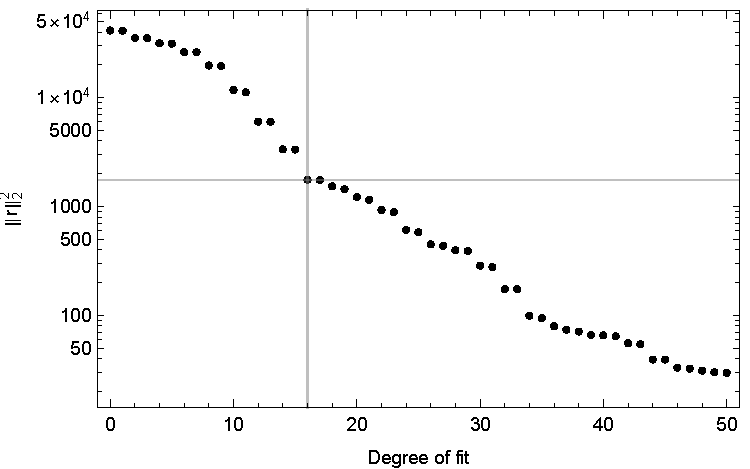
\includegraphics[width=3.2cm]{\pLocalGraphics/nu/nu=16-d=16-C} \\
			%
        \raisebox{1cm}{$50$} &
        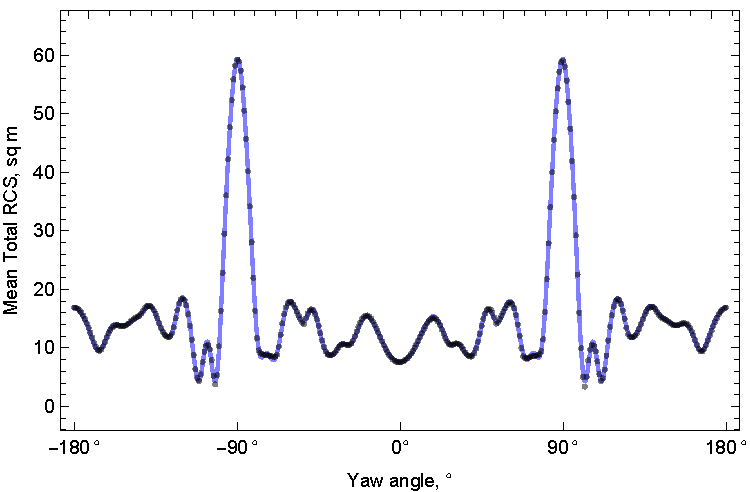
\includegraphics[width=3.1cm]{\pLocalGraphics/nu/nu=16-d=50-A} &
        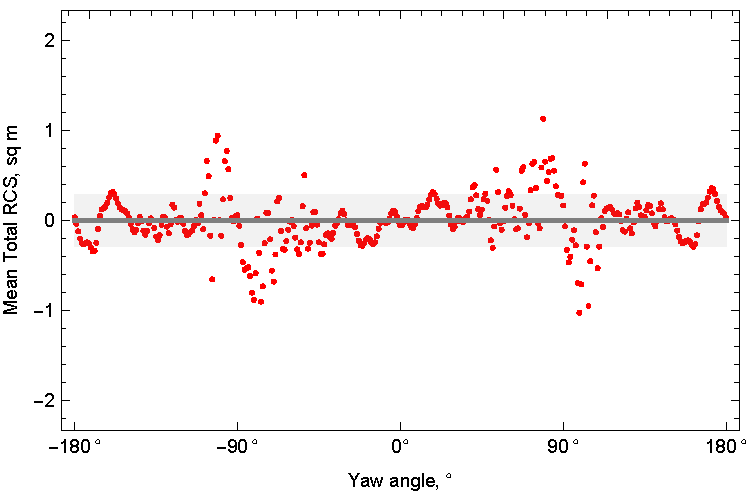
\includegraphics[width=3.1cm]{\pLocalGraphics/nu/nu=16-d=50-B} &
        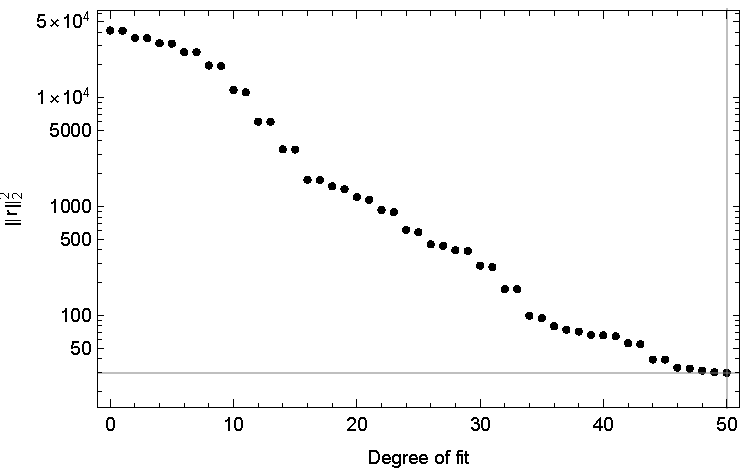
\includegraphics[width=3.2cm]{\pLocalGraphics/nu/nu=16-d=50-C} \\
			%
\end{tabular}
\end{center}
\label{tab:c}
\end{table}%
\end{frame}

%\begin{frame}{A Closer Look}
%    \centering
%    \renewcommand{\arraystretch}{1.2} % Adjust row spacing
%    \setlength{\tabcolsep}{6pt}       % Adjust column spacing
%    
%    % Table Layout
%    \begin{tabular}{>{\centering}m{0.5cm} m{3cm} m{3cm} m{3cm}}
%        % Header Row
%        \textbf{\textit{d}} & \textbf{Data Fit} & \textbf{Residual Error} & \textbf{Total Error} \\\hline
%        % Row 1
%        $16$ &
%        \vspace{0.5em} 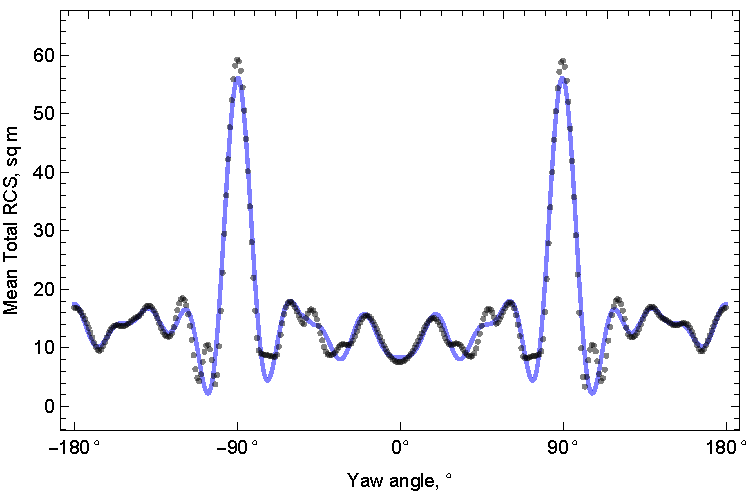
\includegraphics[width=3.1cm]{\pLocalGraphics/nu/nu=16-d=16-A} &
%        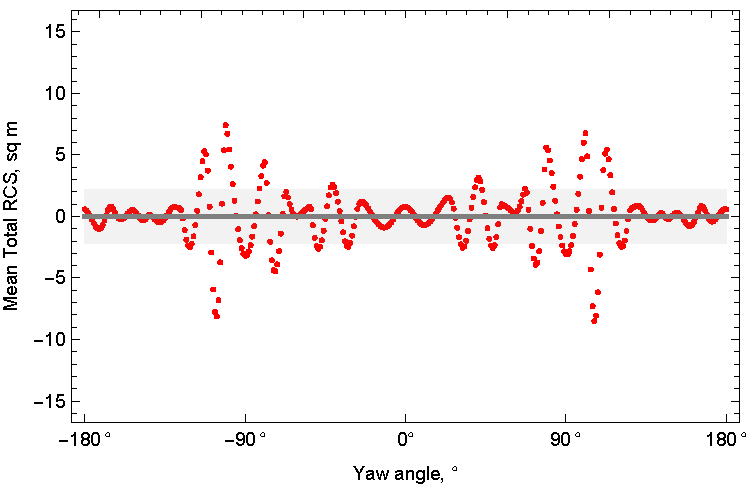
\includegraphics[width=3.1cm]{\pLocalGraphics/nu/nu=16-d=16-B} &
%        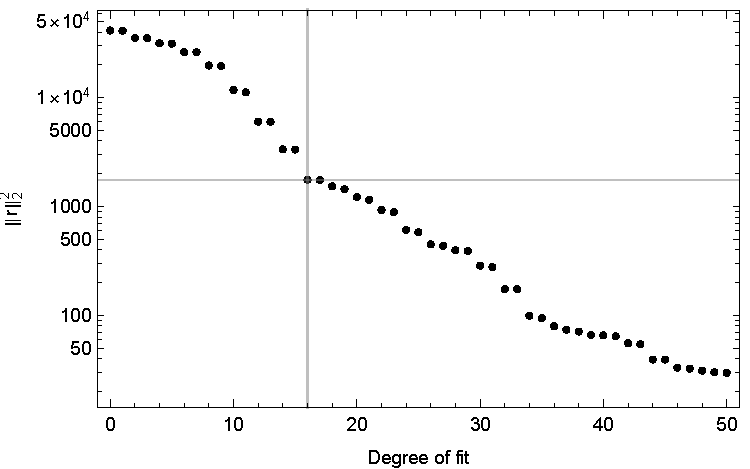
\includegraphics[width=3.1cm]{\pLocalGraphics/nu/nu=16-d=16-C} \\
%        % Row 2
%        $50$ &
%        \vspace{0.5em} 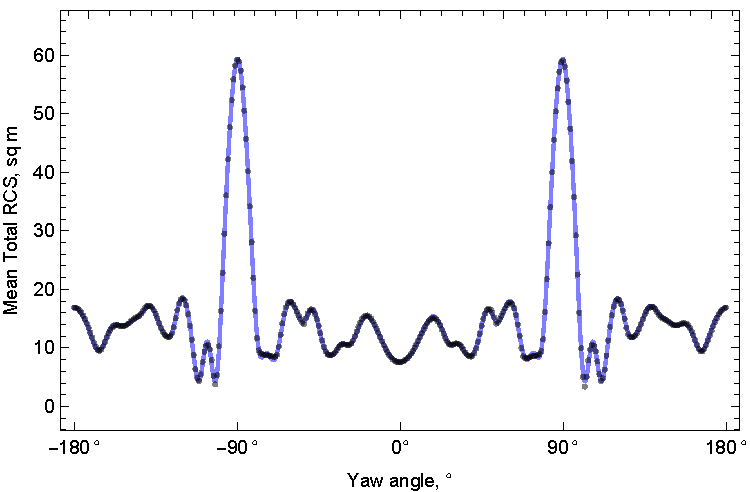
\includegraphics[width=3.1cm]{\pLocalGraphics/nu/nu=16-d=50-A} &
%        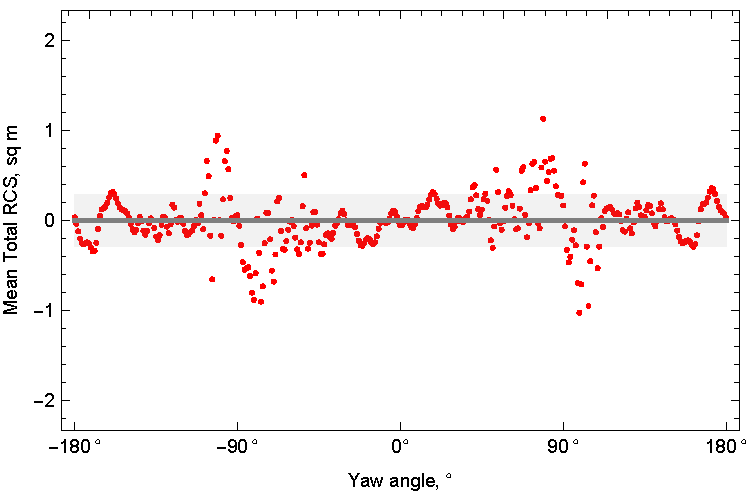
\includegraphics[width=3.1cm]{\pLocalGraphics/nu/nu=16-d=50-B} &
%        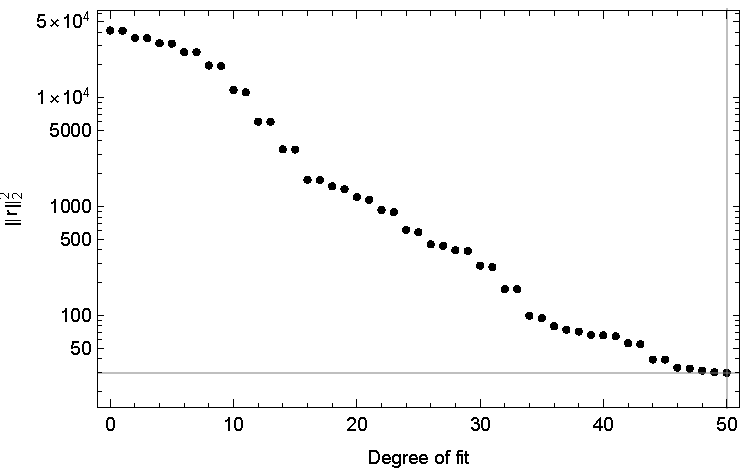
\includegraphics[width=3.1cm]{\pLocalGraphics/nu/nu=16-d=50-C} \\
%    \end{tabular}
%\end{frame}

%\begin{frame}{Fourier Transform Visualizations at 16 MHz}
%    \small
%    \begin{itemize}
%        \item \textcolor{blue}{Approximation Order (\(d\)):} 
%              The number of terms in the Fourier approximation increases as \(d = 1, 2, 4, 8, 16, 24\).
%        \item \textcolor{blue}{Low-Order Approximations:} 
%              Approximations with smaller \(d\) (e.g., \(d = 1, 2, 4\)) fail to capture fine structures, leading to significant residual error.
%        \item \textcolor{blue}{Higher-Order Approximations:} 
%              As \(d\) grows, the approximation better resolves finer features, and the error (gray) shrinks significantly, especially at smooth regions.
%        \item \textcolor{blue}{Error Behavior:} 
%              The error decreases non-uniformly—large errors persist near abrupt changes or peaks due to Gibbs phenomena, but smooth regions converge faster.
%        \item \textcolor{blue}{Key Insight:} 
%              Fourier approximations demonstrate trade-offs: computational complexity increases with \(d\), but fidelity improves.
%        \item \textcolor{blue}{General Notes:}
%              \begin{itemize}
%                  \item Fourier series represent functions as sums of sines and cosines.
%                  \item Low-frequency terms approximate broad trends; high-frequency terms capture fine details.
%                  \item Convergence is faster for smooth functions but slower for discontinuities or sharp changes.
%                  \item Increasing the number of terms improves fidelity but can introduce numerical artifacts if not handled carefully.
%              \end{itemize}
%    \end{itemize}
%\end{frame}

\begin{frame}{Fourier Transform Visualizations at 16 MHz}
    \small
    \begin{itemize}
        \item \textcolor{blue}{Approximation Order (\(d\)):} 
              The number of terms in the Fourier approximation increases as \(d = 1, 2, 4, 8, 16, 24\).
        \item \textcolor{blue}{Low-Order Approximations:} 
              Approximations with smaller \(d\) (e.g., \(d = 1, 2, 4\)) fail to capture fine structures, leading to significant residual error.
        \item \textcolor{blue}{Higher-Order Approximations:} 
              As \(d\) grows, the approximation better resolves finer features, and the error (gray) shrinks significantly, especially at smooth regions.
        \item \textcolor{blue}{Error Behavior:} 
              The error decreases non-uniformly—large errors persist near abrupt changes or peaks due to Gibbs phenomena, but smooth regions converge faster.
    \end{itemize}
\end{frame}

\begin{frame}{Fourier Transform Visualizations at 16 MHz}
    \small
    \begin{itemize}
        \item \textcolor{blue}{Key Insight:} 
              Fourier approximations demonstrate trade-offs: fidelity improves with \(d\), as does computational cost.
        \item \textcolor{blue}{General Notes:}
              \begin{itemize}
                  \item Fourier series resolve functions as sums of sines and cosines.
                  \item Low-frequency terms: broad trends; high-frequency: fine details.
                  \item Convergence is faster for smooth functions but slower for discontinuities or sharp changes.
                  \item More terms improves fidelity, but can introduce numerical artifacts.
              \end{itemize}
    \end{itemize}
\end{frame}


%     %     %     %     %     %     %     %     %
\subsection{Linear Independence}
	
%     %     %     %     %     %     %     %     %
\subsection{Quality of Fit}

\endinput  %  ==  ==  ==  ==  ==  ==  ==  ==  ==
